\chapter{Nature de la lumière et les lois de Snell-Descartes}
\section{Introduction} L'optique nous permet d'étudier la science de la vision, utilisation de la lumière pour les instruments optiques, laser, fibre optiques etc.

La lumière : ce que l'oeil peut voir, le \ul{visible}

\section{Théorie}

\begin{wrapfigure}[6]{r}{0pt}
	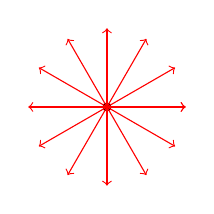
\begin{tikzpicture}
	\draw[fill=black] (0, 0) circle (0.05);
	\foreach \x in {0,30,...,360} 
		\draw[->, red] (0, 0) -- (\x:1cm);
\end{tikzpicture}
\end{wrapfigure}
\subsection{La modèle géométrique}

Il est assez réducteur car se base sur des principes et approximation des propriétés de la lumière :
\begin{itemize}
	\item \ul{Principe} de la propagation rectiligne de la lumière. On parle de \ul{rayon} qui est valable dans un milieu transparent, homogène et isotrope (se propage dans tout les sens).
	\item Le principe de retour inverse de la lumière (Le trajet suivi par la lumière pour aller d'un point à un autre ne dépend pas du sens de propagation de la lumière). 
\end{itemize}

\subsection{Modèle Ondulatoire}

\begin{itemize}
	\item[Huygens] a introduit le phénomène d'onde enveloppe, et la propagation de la lumière de proche en proche.
	\item[Young] a fait l'expérience \ul{d'interference lumineuse} et a démontré que la théorie corpuscule d'Einstein était vrai et a mathématisé le tout. La lumière étaient une onde progressive périodique.
\end{itemize}

\begin{wrapfigure}[3]{r}{0pt}
	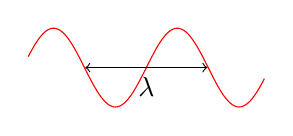
\begin{tikzpicture}[scale=0.5]
		\draw[red, domain=-3:3, samples=300] plot(\x, {sin(2*\x r)});
		\draw[<->] (-1.55, 0) -- (1.55, 0) node [below, midway] {$\lambda$};
	\end{tikzpicture}

\end{wrapfigure}

On utilise ces théorie pour expliquer la diffraction.
Le modèle géométrique s'arrête quand la lumière rencontre des obstacles de même ordre de grandeur que sa longueur d'onde $\lambda$

\ul{Maxwell} dit que la lumière est une onde éléctromagnétique, qui possède de l'énergie et caractérisé par un champ élétrique $\vec{E}$ et magnétique $\vec{B}$.

La vecteur d'onde $\vec{k}$ nous donne la direction de propagation.

La base $(\vec{E}, \vec{B}, \vec{k})$ donne une base orthonormale direct.

\subsection{Corpusculaire}

On tiens compte de cette théorie quand on a une interaction entre la lumière et un atome (des dimensions plus petites que la longueur d'onde caractéristique de la lumière).

\[E = h\nu = \frac{hc}{\lambda} \text{ avec } h \text{ La constante de planque et } \nu \text{ la frequence }\]

\section{Le cadre}

\paragraph{Introduction} Il faut définir le milieu:\begin{itemize}
	\item Le vide la vitesse de la lumière est $c$
	\item La lumière se propage dans un milieu transparent, homogène et isotrope, l'indice de refraction $n$ est défini par : \[n = \frac{c}{v}\] avec c la vitesse de la lumière dans le vide et v dans le milieu étudié. \[\begin{array}{rclr}
	n &=& 1 &\text{dans le vide} \\
	n &=& 1.00029 & \text{dans l'air} \\
	n &=& 1.33 & \text{dans l'eau} \\
	n &=& 1.5 & \text{dans le verre}\end{array}\]
\end{itemize}

La lumière est décrite par les \ul{rayons lumineux} qui forment un faisceau lumineux.

La but de l'optique géométrique est de construire des images. Elle est basé sur les lois de Snell Descartes qui sont les lois de \ul{reflexion} et la loi de \ul{refraction}.

\section{Réflexion et refraction des faisceaux lumineux}
\begin{wrapfigure}[8]{r}{0pt}
	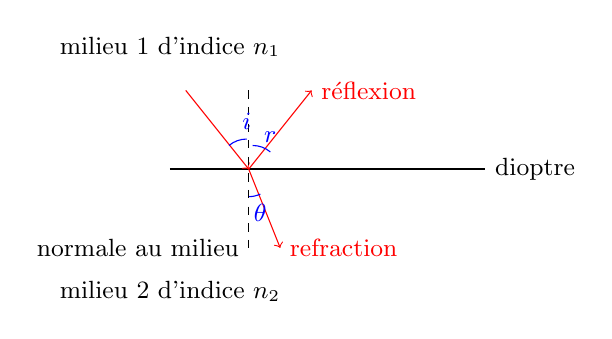
\begin{tikzpicture}[font=\small]
		\node[above] at (0, 1.3) {milieu 1 d'indice $n_1$};
		\node[below] at (0, -1.3) {milieu 2 d'indice $n_2$};
		\draw[thick] (0, 0) -- (4, 0) node[right] {dioptre};
		\draw[red, ->] (0.2, 1) -- (1, 0);
		\draw[red, ->] (1, 0) -- (1.8, 1) node [right] {réflexion};
		\draw[red, ->] (1, 0) -- (1.4, -1) node [right] {refraction};
		\draw[blue] (1, -0.35) arc (270:295:0.35) node [below] {$\theta$};
		\draw[dashed] (1, 1) -- (1, -1) node [left] {normale au milieu};

		\draw[blue] (0.75, 0.3) arc (130:90:0.35) node [above] {$i$};
		\draw[blue] (1.05, 0.3) arc (90:50:0.35) node [above] {$r$};
	\end{tikzpicture}
\end{wrapfigure}

Ces lois s'applique au passage de la lumière d'un milieu 1 dans un milieu 2, ou la surface de séparation est appelé un \ul{dioptre}

\begin{description}
	\item[Reflexion] Le faisceau émergent reste dans le même milieu
	\item[Refraction] Le faisceau émergent change de milieu
	\item[Plan d'incidence] formé par le rayon incident et la normale au milieu.
\end{description}

La rayon réfléchie et coupés dans le plan d'incidence. \[i = r\]
Le rayon réfracté est compris dans le plan d'incidence\[n_1 \sin i = n_2 \sin \theta\]

si $n_2 > n_1$, alors le milieu 2 est plus réfringeant que le milieu 1

\paragraph{Exemple} La lumière passant du verre d'indice $n_1=1.5$ au vide d'indice $n_2=1$. 
\begin{itemize}
	\item pour $i=30^\circ$, $r=48,6^\circ$
	\item pour $i=45^\circ$, le phénomène de réfraction n'existe pas à partir d'un anglais limite $i_2$ qui donne un angle réfracté $r=90^\circ$. Si $i > i_2$, on parle de \ul{reflexion totale} : tout les rayon reste dans le même milieu.

	\item[reflexion total] $n_1 \sin i_1 = n_2 \Rightarrow \sin i_1 = \frac{n_2}{n_1} \Rightarrow i_1 = \arcsin(\frac{1}{1.5}) = 41^\circ$
\end{itemize}

La reflexion total ne peut fonctionner que si on passe dans un milieu \ul{moins refringeant}

\subsection{Principe de retour inverse de la lumière}

Le chemin parcourue est le même en passant pas d'un milieu 1 à un milieu 2 que d'un milieu 2 à milieu 1
